\documentclass[letterpaper]{article}
\usepackage{calc,amsmath,amssymb,amsfonts}
\usepackage[LGR,T1]{fontenc}
\usepackage[greek,spanish,english]{babel}
\usepackage{xcolor,longfbox,multicol,fancyhdr}
\usepackage[top=0.639in,bottom=0.1945in,left=0.5972in,right=0in,noheadfoot]{geometry}
\usepackage{enumitem,hyperref}
\hypersetup{colorlinks=true,allcolors=blue,pdfauthor=Luis Angel Cruz Quispe}
\usepackage[pdftex]{graphicx}
\makeatletter\newdimen\@tempdimd\makeatother
% Outline numbering
\setcounter{secnumdepth}{0}
% Text styles
\newcommand\textstyleStrong[1]{\textbf{#1}}
\newcommand\textstyleHTMLCode[1]{\textrm{#1}}
\newcommand\textstyleEmphasis[1]{\textit{#1}}
% Pages
\fancypagestyle{Standard}{\fancyhf{}
  \fancyhead[L]{}
  \fancyfoot[L]{}
  \renewcommand\headrulewidth{0pt}
  \renewcommand\footrulewidth{0pt}
  \renewcommand\thepage{\arabic{page}}
}
\pagestyle{Standard}
\author{Luis Angel Cruz Quispe}
\date{2024-06-28}
\begin{document}
\clearpage
\pagestyle{Standard}
{\selectlanguage{spanish}\bfseries
Proyecto Final de Fundamentos de Programacio$\acute{}$n}

\begin{center}
\lfbox[margin-right=0.1319in,margin-left=0.1252in,margin-top=0mm,margin-bottom=0mm,border-style=none,padding=0mm,vertical-align=top,raise=-0.9173in]{
\includegraphics[width=2.3472in,height=2.7299in]{a0000-img001.jpg}}
\end{center}

\bigskip
\begin{multicols}{3}
\section{Cruz Quispe Luis Angel}
{\centering\selectlanguage{spanish}
Escuela de Ingeniería Física
\par}

{\centering\selectlanguage{spanish}
\textit{Universidad Nacional de Ingeniería}
\par}

{\centering\selectlanguage{spanish}
\textit{Facultad de Ciencias} \href{mailto:20221664C@uni.pe}{20221664C}
\par}

\section{Rios Cusi Pedro David}
{\centering\selectlanguage{spanish}
Escuela de Ingeniería Física
\par}

{\centering\selectlanguage{spanish}
\textit{Universidad Nacional de Ingeniería}
\par}

{\centering\selectlanguage{spanish}
\textit{Facultad de Ciencias} \href{mailto:20230216J@uni.pe}{20230216J}
\par}


\bigskip

\section{Mamani Benites Jimmy}
{\centering\selectlanguage{spanish}
Escuela de Ingeniería Física
\par}

{\centering\selectlanguage{spanish}
\textit{Universidad Nacional de Ingeniería}
\par}

{\centering\selectlanguage{spanish}
\textit{Facultad de Ciencias }\href{mailto:20211489D@uni.pe}{20211489D}
\par}
\end{multicols}
\begin{multicols}{2}

\bigskip


\bigskip

{\selectlanguage{spanish}
\textbf{\textit{Resu}}\textbf{\textsc{m}}\textbf{\textit{en}}\textbf{$\text{\textgreek{—}}$} \textbf{Este proyecto
explora el análisis de datos, machine learning y visualización utilizando las bibliotecas de Python Pandas, Matplotlib
y NumPy. Pandas facilita la manipulación de datos tabulares, Matplotlib permite crear diversos gráficos, y NumPy es
fundamental para operaciones numéricas eficientes. Se incluyen ejercicios prácticos que demuestran la integración y
aplicabilidad de estas herramientas en el análisis y visualización de datos.}}


\bigskip


\bigskip

{\selectlanguage{spanish}
I.\ \ INTRODUCCION}

{\selectlanguage{spanish}
\foreignlanguage{spanish}{Este proyecto explora herramientas y técnicas clave de análisis de datos, machine learning,
procesamiento de lenguaje natural, desarrollo web y automatización. Utilizamos las librerías de Python Pandas,
Matplotlib y NumPy para la manipulación y visualización de datos.}}


\bigskip


\bigskip


\bigskip


\bigskip


\bigskip


\bigskip


\bigskip


\bigskip


\bigskip


\bigskip


\bigskip


\bigskip


\bigskip


\bigskip


\bigskip


\bigskip

{\selectlanguage{spanish}
II.\ \ MARCO \ TEORICO}

{\selectlanguage{spanish}
\textit{II-A. \ \ Librerías}}

{\selectlanguage{spanish}
\foreignlanguage{spanish}{\textbf{\textit{{Panda}}}}\foreignlanguage{spanish}{\textbf{\textit{:}}}}

{\selectlanguage{spanish}
\foreignlanguage{spanish}{Es una biblioteca de análisis de datos que proporciona estructuras de datos de alto nivel y
herramientas para trabajar con datos estructurados o tabulares. Aquí están los puntos clave:}}


\bigskip

\begin{enumerate}[series=listWWNumiv,label=\Roman*.,ref=\Roman*]
\item {\selectlanguage{spanish}
\foreignlanguage{spanish}{\textbf{{Dataframe}}}\foreignlanguage{spanish}{\textbf{:}}\foreignlanguage{spanish}{
Es la estructura central en Pandas, que representa datos en forma de tablas con filas y columnas etiquetadas. Los
DataFrames permiten manipular datos de manera similar a una hoja de cálculo.}}
\item {\selectlanguage{spanish}
\foreignlanguage{spanish}{\textbf{{Series}}}\foreignlanguage{spanish}{\textbf{:}}\foreignlanguage{spanish}{
Es otra estructura importante en Pandas, que representa una columna unidimensional en un DataFrame, junto con un
índice.}}
\item {\selectlanguage{spanish}
\foreignlanguage{spanish}{\textbf{{Operaciones de
datos}}}\foreignlanguage{spanish}{\textbf{:}}\foreignlanguage{spanish}{ Pandas ofrece funcionalidades poderosas para
limpiar, transformar, fusionar y analizar datos. Esto incluye manipulaciones de datos como filtros, agregaciones,
agrupaciones y pivoteo.}}
\end{enumerate}

\bigskip


\bigskip


\bigskip


\bigskip


\bigskip


\bigskip


\bigskip


\bigskip


\bigskip


\bigskip

{\selectlanguage{spanish}
\textit{II-B. \ \ Librerías}}

{\selectlanguage{spanish}
\foreignlanguage{spanish}{\textbf{\textit{{Matplotlib}}}}\foreignlanguage{spanish}{\textbf{\textit{:}}}}

{\selectlanguage{spanish}
\foreignlanguage{spanish}{Es la biblioteca estándar para visualización de datos en Python. Ofrece una variedad de
funciones para crear gráficos estáticos, gráficos interactivos, subplots y más. }Los aspectos destacados son:}


\bigskip

\begin{enumerate}[series=listWWNumv,label=\Roman*.,ref=\Roman*]
\item {\selectlanguage{spanish}
\textstyleStrong{\foreignlanguage{spanish}{{Estilos de gráficos}}}\foreignlanguage{spanish}{:
Permite crear una amplia gama de gráficos, incluyendo gráficos \ \ de líneas, barras, dispersión, histogramas,
diagramas de caja y más.}}
\item {\selectlanguage{spanish}
\textstyleStrong{\foreignlanguage{spanish}{\{Personalización}}}\foreignlanguage{spanish}{: Ofrece
control completo sobre la apariencia de los gráficos, incluyendo colores, marcadores, leyendas, etiquetas de ejes y
títulos.}}
\item {\selectlanguage{spanish}
\textstyleStrong{\foreignlanguage{spanish}{{Subplots y figuras
multiples}}}\foreignlanguage{spanish}{: Permite crear múltiples gráficos dentro de la misma figura y personalizar su
disposición.}}
\item {\selectlanguage{spanish}
\textstyleStrong{\foreignlanguage{spanish}{{Interactividad}}}\foreignlanguage{spanish}{: A
través de otras bibliotecas como }\textstyleHTMLCode{\foreignlanguage{spanish}{mpld3}}\foreignlanguage{spanish}{ o
}\textstyleHTMLCode{\foreignlanguage{spanish}{Plotly}}\foreignlanguage{spanish}{, Matplotlib puede ser utilizada para
crear gráficos interactivos y widgets en notebooks de Jupyter.}}
\end{enumerate}

\bigskip

{\selectlanguage{spanish}
\textit{II-C. \ \ Librerías}}

{\selectlanguage{spanish}
\foreignlanguage{spanish}{\textbf{{Numpy}}}\foreignlanguage{spanish}{\textbf{:}}}

{\selectlanguage{spanish}
\foreignlanguage{spanish}{Es la biblioteca fundamental para la computación científica en Python. Proporciona soporte
para arrays multidimensionales (llamados
}\textstyleHTMLCode{\foreignlanguage{spanish}{ndarray}}\foreignlanguage{spanish}{), junto con una amplia colección de
funciones matemáticas para operar en estos arrays. }Algunos conceptos clave incluyen:}


\bigskip

\begin{enumerate}[series=listWWNumvi,label=\Roman*.,ref=\Roman*]
\item {\selectlanguage{spanish}
\foreignlanguage{spanish}{\textbf{{Arrays}}}\foreignlanguage{spanish}{\textbf{:
}}\foreignlanguage{spanish}{Son estructuras de datos fundamentales en NumPy, que permiten almacenar datos de manera
eficiente y realizar operaciones vectorizadas.}}
\item {\selectlanguage{spanish}
\textstyleStrong{\foreignlanguage{spanish}{{Operaciones
vectorizadas}}}\foreignlanguage{spanish}{: NumPy permite realizar operaciones rápidas en arrays completos sin necesidad
de bucles explícitos, lo cual es crucial para la eficiencia en el procesamiento de datos.}}
\item {\selectlanguage{spanish}
\textstyleStrong{\foreignlanguage{spanish}{{Funciones matemáticas}}}\foreignlanguage{spanish}{:
Proporciona funciones para operaciones matemáticas }}
\item {\selectlanguage{spanish}
\foreignlanguage{spanish}{básicas y avanzadas, como funciones trigonométricas, álgebra lineal, estadísticas y más.}}
\item {\selectlanguage{spanish}
\textstyleStrong{\foreignlanguage{spanish}{Indexación y segmentación
avanzadas}}}\foreignlanguage{spanish}{: Permite acceder y manipular datos dentro de arrays utilizando técnicas
poderosas de indexación y segmentación.}}
\end{enumerate}

\bigskip


\bigskip


\bigskip


\bigskip


\bigskip


\bigskip


\bigskip


\bigskip


\bigskip


\bigskip


\bigskip


\bigskip


\bigskip


\bigskip


\bigskip



{\selectlanguage{spanish}
III.\ \ DESARROLLO}

{\selectlanguage{spanish}
\foreignlanguage{spanish}{Aquí haremos presencia de los códigos de los respectivos de los ejercicios planteados en los
cuadernos compartidos en github:}}


\bigskip

\begin{enumerate}[series=listWWNumiii,label=\arabic*.,ref=\arabic*]
\item \begin{enumerate}[series=listWWNumiii,label=\arabic{enumi}.\arabic*]
\item {\selectlanguage{spanish}
\foreignlanguage{spanish}{Ejercicios del cuaderno de Pandas:}}
\end{enumerate}
\end{enumerate}


{\selectlanguage{spanish}
\foreignlanguage{spanish}{\ 3.1.1}}

\begin{center}
\lfbox[margin-right=0.1252in,margin-left=0.1252in,margin-top=0mm,margin-bottom=0mm,border-style=none,padding=0mm,vertical-align=top,raise=-0.1835in]{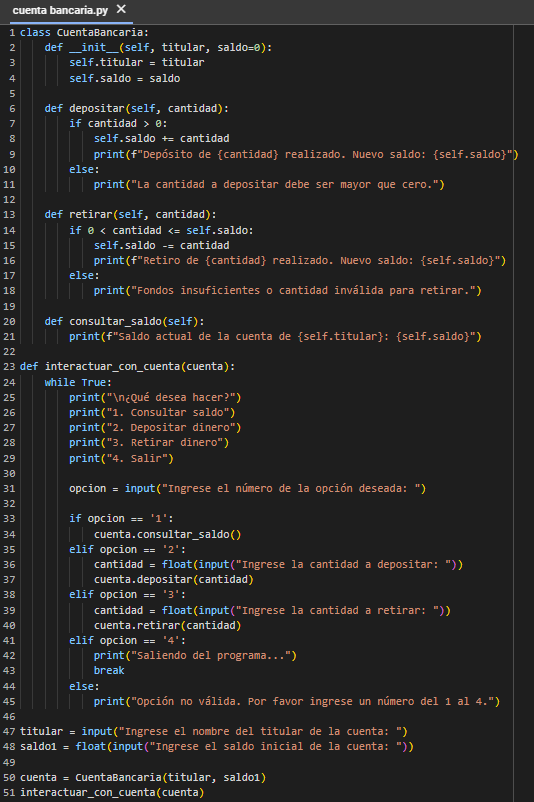
\includegraphics[width=3.5492in,height=2.7362in]{a0000-img003.png}}
\lfbox[margin-right=0.1252in,margin-bottom=0.0028in,margin-left=0.1252in,margin-top=0mm,border-style=none,padding=0mm,vertical-align=top,raise=-3.1398in]{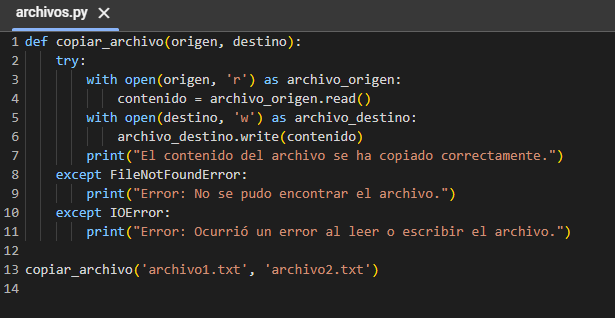
\includegraphics[width=3.5492in,height=0.8098in]{a0000-img002.png}}
\end{center}
\begin{center}

\end{center}

\bigskip


\bigskip


\bigskip


\bigskip


\bigskip


\bigskip


\bigskip


\bigskip


\bigskip


\bigskip


\bigskip


\bigskip


\bigskip


\bigskip


\bigskip


\bigskip


\bigskip


\bigskip

{\selectlanguage{spanish}
\foreignlanguage{spanish}{3.1.}\foreignlanguage{spanish}{2}}
\begin{center}
\lfbox[margin-right=0.1319in,margin-left=0.1252in,margin-top=0mm,margin-bottom=0mm,border-style=none,padding=0mm,vertical-align=top,raise=-0.4102in]{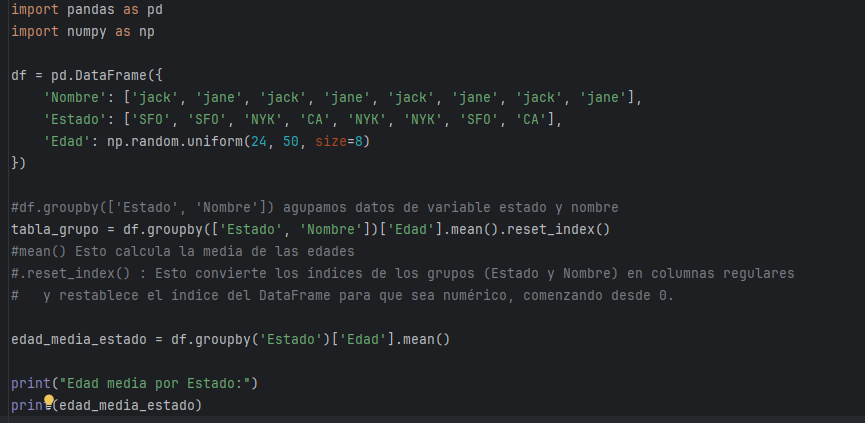
\includegraphics[width=3.4307in,height=1.6764in]{a0000-img005.png}}
\end{center}
\begin{center}
\lfbox[margin-right=0.1252in,margin-left=0.1252in,margin-top=0mm,margin-bottom=0mm,border-style=none,padding=0mm,vertical-align=top,raise=-2.3346in]{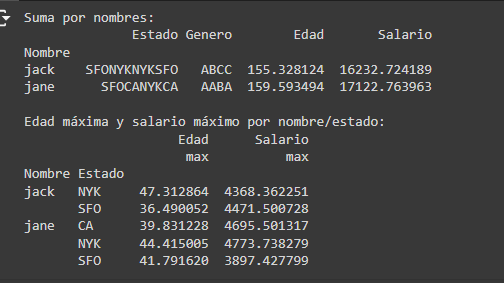
\includegraphics[width=3.4181in,height=1.9181in]{a0000-img004.png}}
\end{center}


\bigskip


\bigskip


\bigskip


\bigskip


\bigskip


\bigskip


\bigskip


\bigskip


\bigskip


\bigskip


\bigskip


\bigskip


\bigskip


\bigskip


\bigskip


\bigskip


\bigskip


\bigskip


\bigskip


\bigskip


\bigskip


\bigskip


\bigskip


\bigskip


\bigskip


\bigskip


\bigskip


\bigskip


\bigskip


\bigskip


\bigskip
\bigskip
{\selectlanguage{spanish}
\foreignlanguage{spanish}{3.1.}\foreignlanguage{spanish}{3}}\begin{center}
\lfbox[margin-right=0.1311in,margin-left=0.1252in,margin-top=0mm,margin-bottom=0mm,border-style=none,padding=0mm,vertical-align=top,raise=-0.4161in]{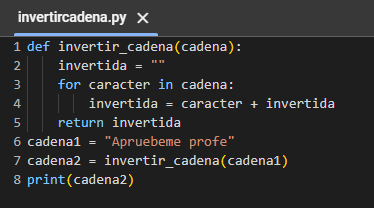
\includegraphics[width=3.702in,height=2.1457in]{a0000-img006.png}}\end{center}\begin{center}
\lfbox[margin-right=0.1291in,margin-left=0.1252in,margin-top=0mm,margin-bottom=0mm,border-style=none,padding=0mm,vertical-align=top,raise=-2.478in]{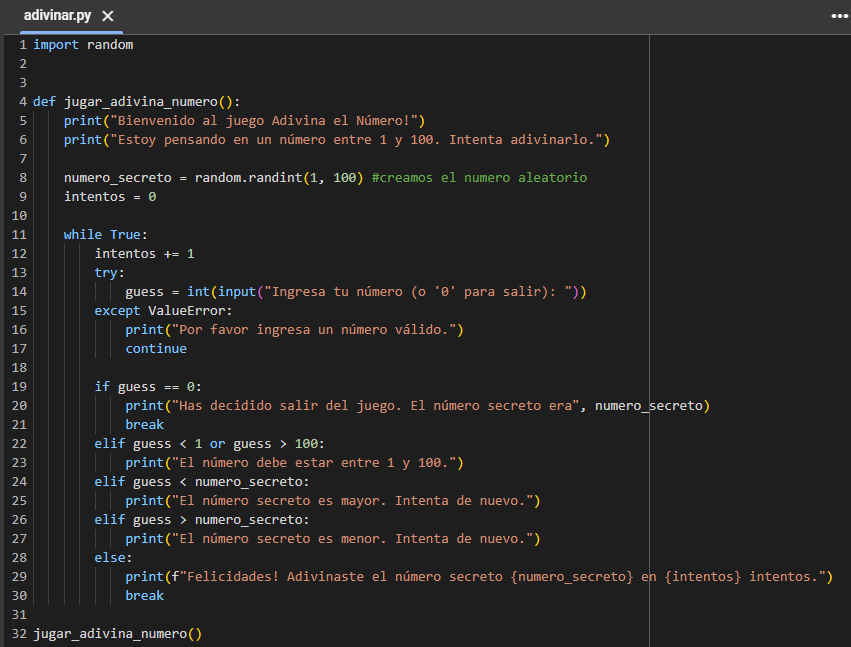
\includegraphics[width=3.6209in,height=1.3835in]{a0000-img007.png}}
\end{center}

\bigskip


\bigskip


\bigskip


\bigskip


\bigskip


\bigskip


\bigskip


\bigskip


\bigskip


\bigskip


\bigskip


\bigskip


\bigskip


\bigskip


\bigskip


\bigskip

{\selectlanguage{spanish}
\foreignlanguage{spanish}{3.2 Ejercicios del cuaderno de Numpy:}}


\bigskip

{\selectlanguage{spanish}
\foreignlanguage{spanish}{3.2.1}
\lfbox[margin-right=0.0091in,margin-top=0mm,margin-bottom=0mm,margin-left=0mm,border-style=none,padding=0mm,vertical-align=top]{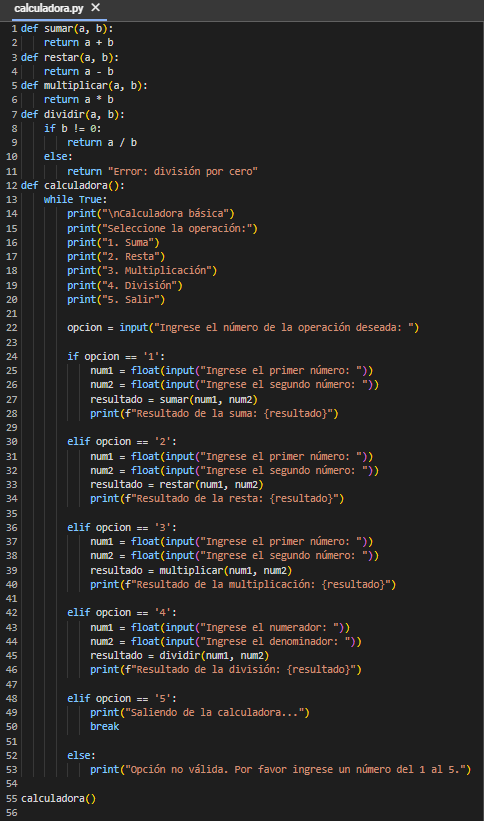
\includegraphics[width=3.1366in,height=3.8791in]{a0000-img008.png}}
}


\bigskip


\lfbox[margin-right=0.0091in,margin-top=0mm,margin-bottom=0mm,margin-left=0mm,border-style=none,padding=0mm,vertical-align=top]{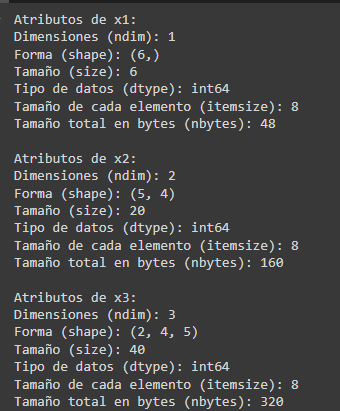
\includegraphics[width=3.1366in,height=3.7917in]{a0000-img009.png}}



\bigskip


\bigskip


\bigskip


\bigskip


\bigskip


\bigskip


\bigskip


\bigskip


\bigskip


\bigskip


\bigskip


\bigskip


\bigskip

{\selectlanguage{spanish}
\foreignlanguage{spanish}{3.2.2}}


\lfbox[margin=0mm,border-style=none,padding=0mm,vertical-align=top]{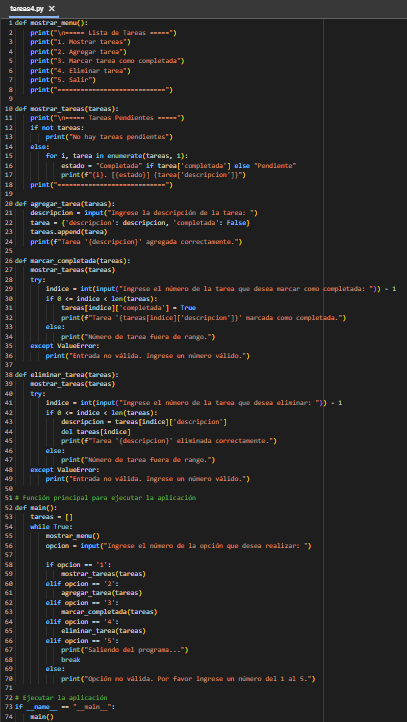
\includegraphics[width=3.6937in,height=2.8547in]{a0000-img010.png}}



\bigskip


\lfbox[margin=0mm,border-style=none,padding=0mm,vertical-align=top]{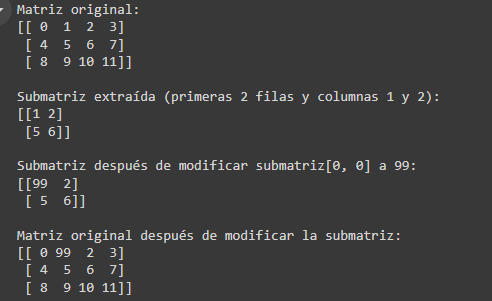
\includegraphics[width=3.6937in,height=2.2598in]{a0000-img011.png}}



\bigskip


\bigskip


\bigskip


\bigskip


\bigskip


\bigskip


\bigskip


\bigskip


\bigskip


\bigskip


\bigskip


\bigskip


\bigskip


\bigskip


\bigskip


\bigskip


\bigskip


\bigskip


\bigskip


\bigskip


\bigskip


\bigskip


\bigskip


\bigskip


\bigskip


\bigskip


\bigskip


\bigskip


\bigskip


\bigskip


\bigskip


\bigskip


\bigskip


\bigskip


\bigskip


\bigskip


\bigskip

{\selectlanguage{spanish}
\foreignlanguage{spanish}{3.3 Ejercicios del cuaderno de matplotlib:}}

{\selectlanguage{spanish}
\foreignlanguage{spanish}{3.3.1}

\lfbox[margin=0mm,border-style=none,padding=0mm,vertical-align=top]{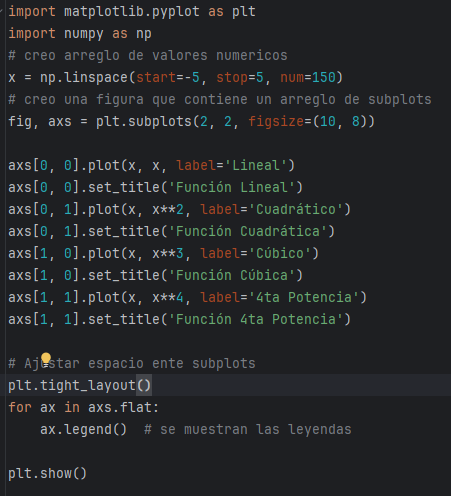
\includegraphics[width=3.2071in,height=3.5272in]{a0000-img012.png}}
 }

\lfbox[margin=0mm,border-style=none,padding=0mm,vertical-align=top]{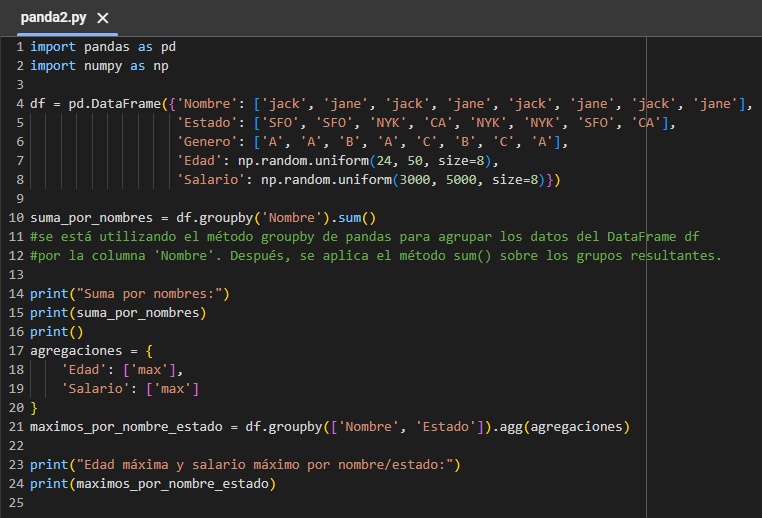
\includegraphics[width=3.2102in,height=2.5228in]{a0000-img013.png}}



\bigskip


\bigskip


\bigskip


\bigskip


\bigskip


\bigskip


\bigskip


\bigskip


\bigskip


\bigskip


\bigskip


\bigskip


\bigskip


\bigskip


\bigskip


\bigskip


\bigskip


\bigskip


\bigskip


\bigskip


\bigskip


\bigskip


\bigskip


\bigskip


\bigskip


\bigskip


\bigskip


\bigskip


\bigskip


\bigskip


\bigskip


\bigskip


\bigskip

{\selectlanguage{spanish}
\foreignlanguage{spanish}{3.3.2}
\bigskip
\lfbox[margin=0mm,border-style=none,padding=0mm,vertical-align=top]{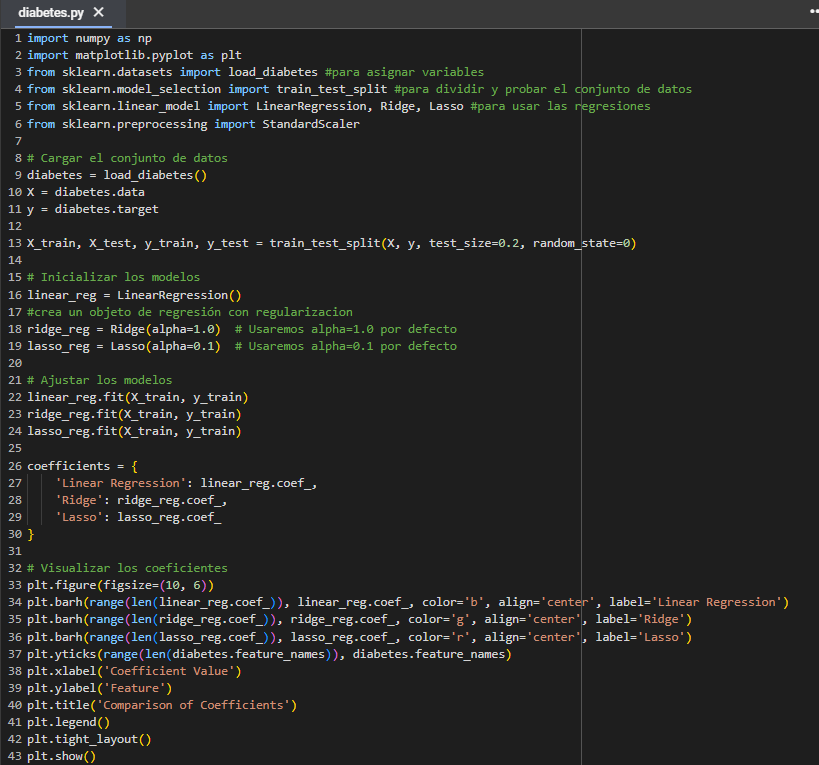
\includegraphics[width=3.5634in,height=1.2917in]{a0000-img014.png}}
}


\bigskip


\lfbox[margin=0mm,border-style=none,padding=0mm,vertical-align=top]{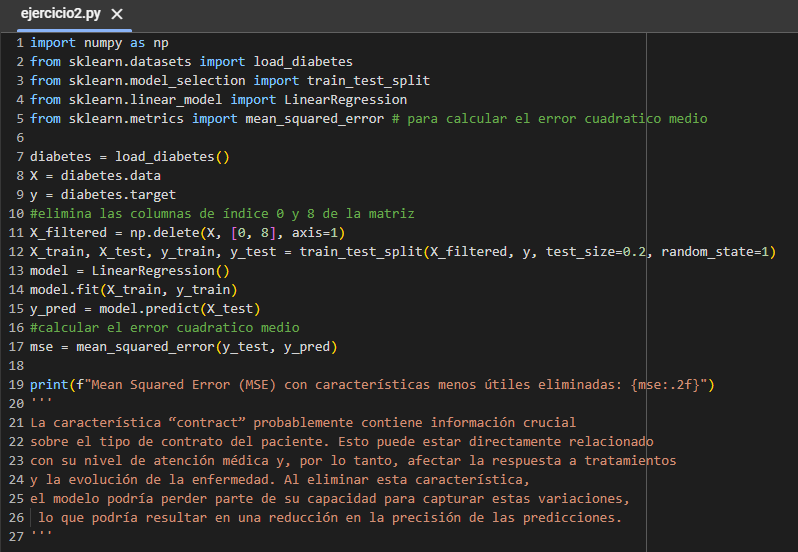
\includegraphics[width=3.5626in,height=2.5665in]{a0000-img015.png}}



\bigskip


\bigskip


\bigskip


\bigskip


\bigskip


\bigskip


\bigskip


\bigskip


\bigskip


\bigskip


\bigskip


\bigskip


\bigskip


\bigskip


\bigskip


\bigskip


\bigskip


\bigskip


\bigskip


\bigskip


\bigskip


\bigskip


\bigskip


\bigskip


\bigskip


\bigskip


\bigskip

\bigskip
\bigskip
\bigskip
\bigskip
\bigskip

{\selectlanguage{spanish}
\bigskip
\bigskip
\bigskip
\bigskip
\bigskip
\foreignlanguage{spanish}{3.3.3} }


\lfbox[margin=0mm,border-style=none,padding=0mm,vertical-align=top]{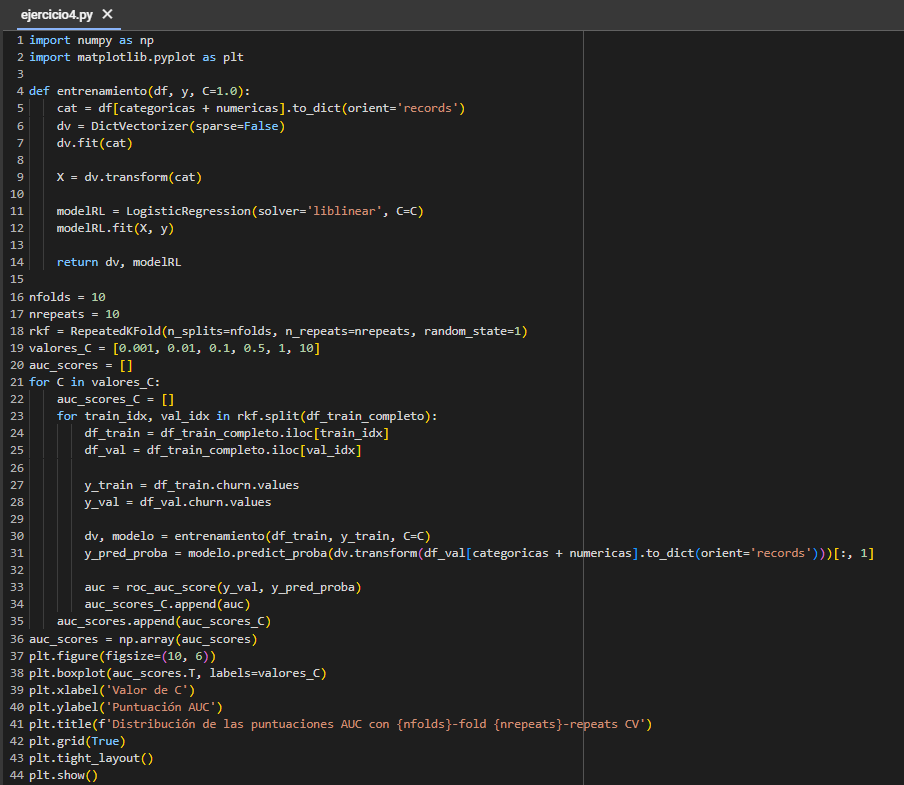
\includegraphics[width=3.5654in,height=1.872in]{a0000-img016.png}}



\bigskip


\lfbox[margin=0mm,border-style=none,padding=0mm,vertical-align=top]{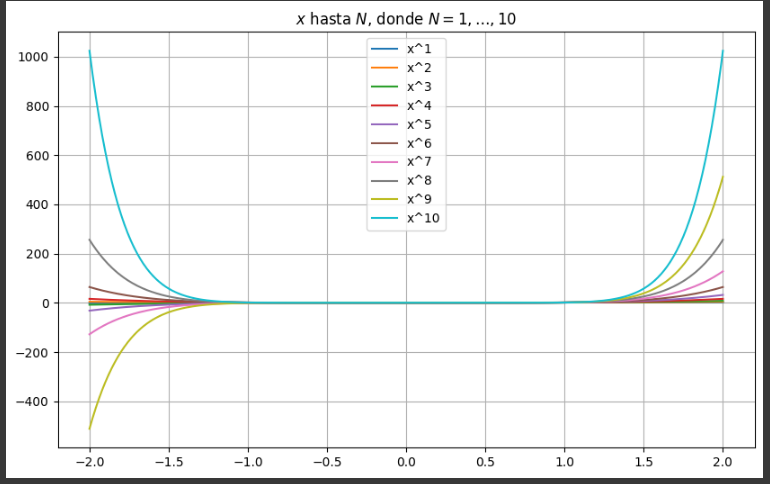
\includegraphics[width=3.5646in,height=1.8154in]{a0000-img017.png}}



\bigskip


\bigskip


\bigskip


\bigskip


\bigskip


\bigskip


\bigskip


\bigskip


\bigskip


\bigskip


\bigskip


\bigskip


\bigskip


\bigskip


\bigskip


\bigskip


\bigskip


\bigskip


\bigskip


\bigskip


\bigskip


\bigskip


\bigskip


\bigskip


\bigskip


\bigskip


\bigskip

{\selectlanguage{spanish}
\bigskip
\bigskip
\bigskip
\bigskip
\bigskip
\bigskip
\bigskip
\bigskip
\bigskip
\bigskip
\bigskip
\bigskip
\bigskip
\bigskip
\bigskip
\bigskip
\bigskip
\bigskip
\bigskip
\bigskip
\bigskip









\bigskip
\bigskip
\bigskip
\bigskip
\bigskip
\bigskip
\bigskip
\bigskip
\bigskip
\bigskip
\bigskip
\bigskip
\bigskip
\bigskip
\bigskip
\foreignlanguage{spanish}
\bigskip
\bigskip
\bigskip
\bigskip
\bigskip
\bigskip
\bigskip
\bigskip
{3.3.4}}
\lfbox[margin=0mm,border-style=none,padding=0mm,vertical-align=top]{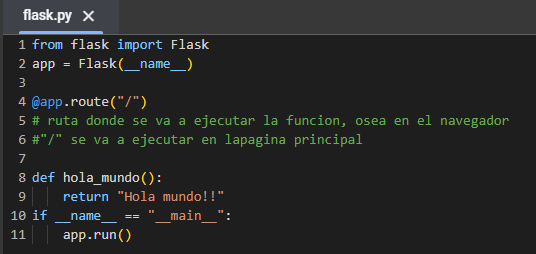
\includegraphics[width=3.9409in,height=2.2126in]{a0000-img018.png}}
\lfbox[margin-right=0.0055in,margin-bottom=0.0063in,margin-top=0mm,margin-left=0mm,border-style=none,padding=0mm,vertical-align=top]{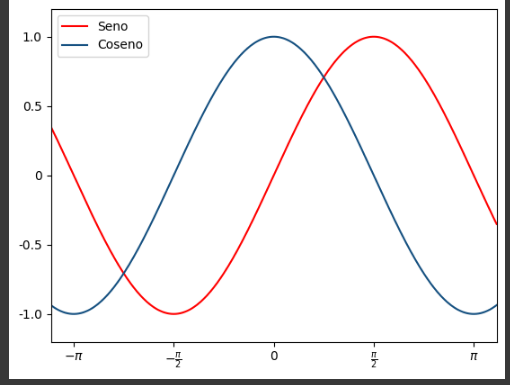
\includegraphics[width=3.828in,height=2.8898in]{a0000-img019.png}}



\bigskip


\bigskip


\bigskip


\bigskip


\bigskip


\bigskip


\bigskip


\bigskip


\bigskip


\bigskip


\bigskip


\bigskip


\bigskip


\bigskip


\bigskip


\bigskip


\bigskip


\bigskip


\bigskip


\bigskip


\bigskip


\bigskip


\bigskip


\bigskip


\bigskip


\bigskip


\bigskip


\bigskip


\bigskip


\bigskip


\bigskip


\bigskip


\bigskip


\bigskip


\bigskip

{\selectlanguage{spanish}
\foreignlanguage{spanish}{3.3.5}}


\lfbox[margin=0mm,border-style=none,padding=0mm,vertical-align=top]{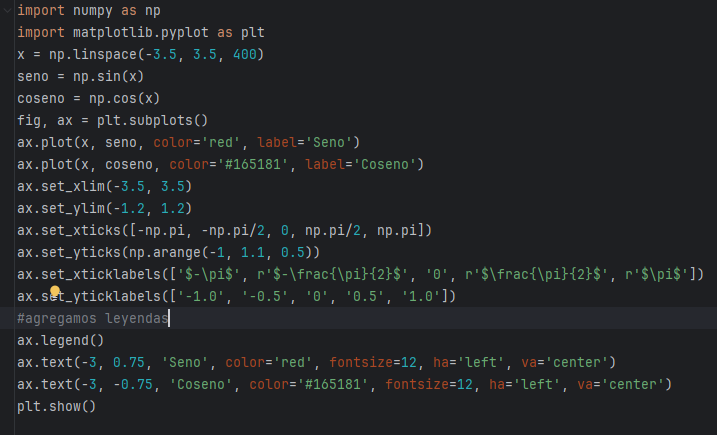
\includegraphics[width=3.5846in,height=2.1744in]{a0000-img020.png}}



\lfbox[margin=0mm,border-style=none,padding=0mm,vertical-align=top]{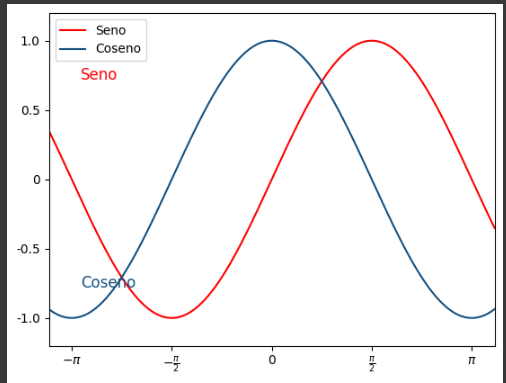
\includegraphics[width=3.5839in,height=2.7134in]{a0000-img021.png}}



\bigskip


\bigskip


\bigskip


\bigskip


\bigskip


\bigskip


\bigskip


\bigskip


\bigskip


\bigskip


\bigskip


\bigskip


\bigskip


\bigskip


\bigskip


\bigskip


\bigskip


\bigskip


\bigskip


\bigskip


\bigskip


\bigskip


\bigskip


\bigskip
\bigskip
\bigskip
\bigskip
\bigskip
\bigskip
\bigskip
\bigskip
\bigskip
{\selectlanguage{spanish}
\foreignlanguage{spanish}{3.3.6}}


\lfbox[margin-right=0.0016in,margin-bottom=0.0055in,margin-top=0mm,margin-left=0mm,border-style=none,padding=0mm,vertical-align=top]{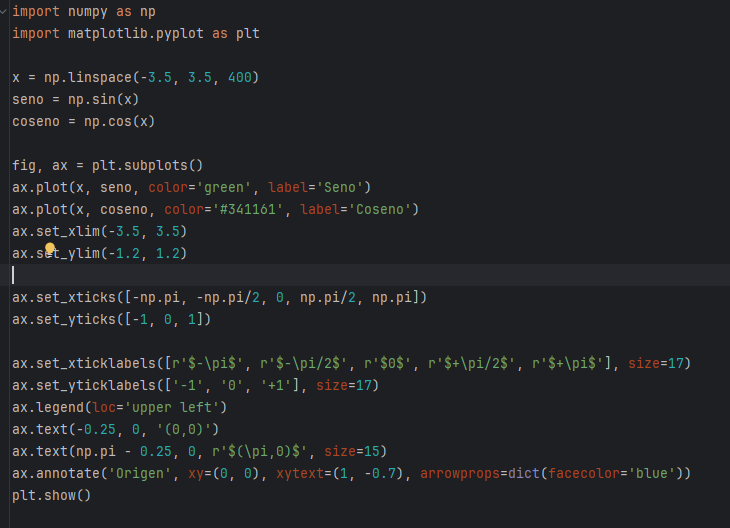
\includegraphics[width=3.8528in,height=2.7866in]{a0000-img022.png}}



\bigskip


\lfbox[margin-right=0.002in,margin-top=0mm,margin-bottom=0mm,margin-left=0mm,border-style=none,padding=0mm,vertical-align=top]{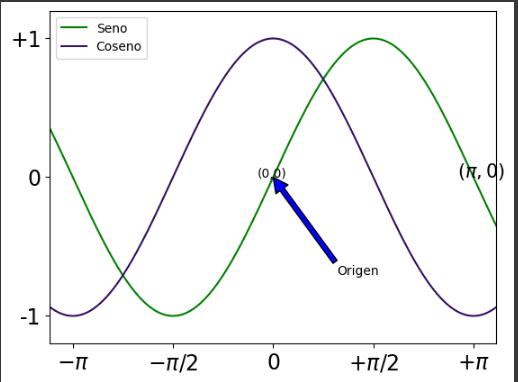
\includegraphics[width=3.852in,height=2.8409in]{a0000-img023.png}}



\bigskip


\bigskip


\bigskip


\bigskip


\bigskip


\bigskip


\bigskip


\bigskip


\bigskip


\bigskip


\bigskip


\bigskip


\bigskip


\bigskip


\bigskip


\bigskip


\bigskip


\bigskip


\bigskip


\bigskip


\bigskip


\bigskip


\bigskip


\bigskip


\bigskip


\bigskip


\bigskip


\bigskip


\bigskip


\bigskip


\bigskip


\bigskip


\bigskip


\bigskip


\bigskip


\bigskip


\bigskip

{\selectlanguage{spanish}
\foreignlanguage{spanish}{3.3.7}}


\lfbox[margin-right=0.0043in,margin-top=0mm,margin-bottom=0mm,margin-left=0mm,border-style=none,padding=0mm,vertical-align=top]{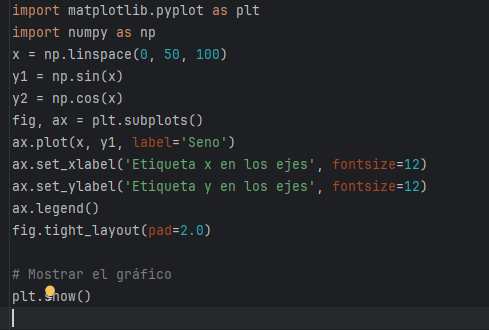
\includegraphics[width=3.2882in,height=2.2189in]{a0000-img024.png}}



\bigskip


\lfbox[margin=0mm,border-style=none,padding=0mm,vertical-align=top]{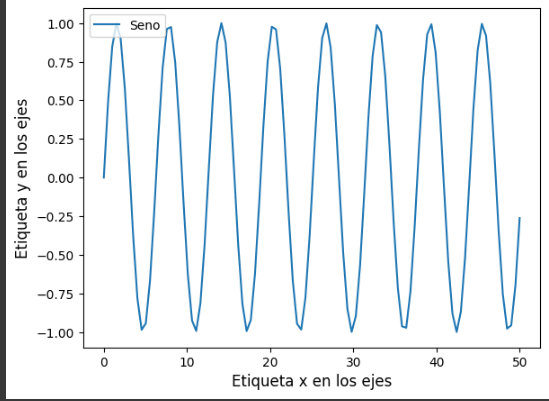
\includegraphics[width=3.5457in,height=2.5898in]{a0000-img025.png}}



\bigskip


\bigskip


\bigskip


\bigskip

{\selectlanguage{spanish}
I.\ \ CONCLUSIONES}

{\selectlanguage{spanish}
\foreignlanguage{spanish}{En conclusión, las bibliotecas NumPy, Pandas y Matplotlib se presentan como pilares
fundamentales en el ecosistema de Python para el análisis de datos y la visualización. }}


\bigskip

{\selectlanguage{spanish}
\foreignlanguage{spanish}{NumPy proporciona la base eficiente para operaciones numéricas en arrays multidimensionales,
esencial para el procesamiento de datos a gran escala. Por otro lado, Pandas simplifica significativamente la
manipulación y el análisis de datos tabulares mediante sus estructuras de datos flexibles como DataFrames y Series,
permitiendo operaciones complejas con facilidad. }}


\bigskip

{\selectlanguage{spanish}
\foreignlanguage{spanish}{Finalmente, Matplotlib destaca por su capacidad para crear una amplia variedad de gráficos
estáticos y interactivos, ofreciendo control detallado sobre la apariencia visual de los datos. }}


\bigskip

{\selectlanguage{spanish}
\foreignlanguage{spanish}{La integración fluida entre estas bibliotecas facilita un flujo de trabajo coherente y
eficiente desde la carga de datos hasta su análisis y visualización, convirtiéndolas en herramientas indispensables
para cualquier profesional o investigador que trabaje con datos en Python.}}


\bigskip


\bigskip

{\selectlanguage{spanish}
\foreignlanguage{english}{V.\ \ BIBLIOGRAFÍA}}


\bigskip

{\selectlanguage{spanish}
\foreignlanguage{english}{McKinney, W. (2017). }\textstyleEmphasis{\foreignlanguage{english}{Python for Data Analysis:
Data Wrangling with Pandas, NumPy, and IPython}}\foreignlanguage{english}{. O'Reilly Media.}}


\bigskip

{\selectlanguage{spanish}
\foreignlanguage{english}{The pandas development team. (2020).
}\textstyleEmphasis{\foreignlanguage{english}{pandas-dev/pandas: Pandas}}\foreignlanguage{english}{. Zenodo.
doi:10.5281/zenodo.3509134}}


\bigskip

{\selectlanguage{spanish}
\foreignlanguage{english}{The matplotlib development team. (2020).
}\textstyleEmphasis{\foreignlanguage{english}{matplotlib/matplotlib: Matplotlib}}\foreignlanguage{english}{. Zenodo.
doi:10.5281/zenodo.3893257}}
\end{multicols}
\end{document}
